\documentclass[dvipdfmx]{jarticle}
    \usepackage{graphicx}
    \usepackage[ top=25truemm,bottom=37truemm,left=25truemm,right=25truemm]
    {geometry}
    \usepackage{ascmac}
    \usepackage{array}
    \usepackage{here}
    \usepackage{url}
    \usepackage{listings, jlisting}
    \usepackage{tikz}
    \usepackage{cases}
    \usetikzlibrary{intersections,calc,arrows}
    \renewcommand{\lstlistingname}{リスト}
\lstset{language=c,
  basicstyle=\ttfamily\scriptsize,
  commentstyle=\textit,
  classoffset=1,
  keywordstyle=\bfseries,
  frame=tRBl,
  framesep=5pt,
  showstringspaces=false,
  numbers=left,
  stepnumber=1,
  numberstyle=\tiny,
  tabsize=4
}

\makeatletter
\def\@thesis{シミュレーション レポート}
\def\id#1{\def\@id{#1}}
\def\department#1{\def\@department{#1}}

\def\@maketitle{
\begin{center}
{\huge \@thesis \par} %修士論文と記載される部分
\vspace{10mm}
{\LARGE\bf \@title \par}% 論文のタイトル部分
\vspace{10mm}
{\Large \@date\par}	% 提出年月日部分
\vspace{20mm}
{\Large \@department \par}	% 所属部分
{\Large 学籍番号 \@id \par}	% 学籍番号部分
\vspace{10mm}
{\Large 氏名 \@author}% 氏名 
\end{center}
\par\vskip 1.5em
}

\title{第1回~第5回}
\date{提出期限 2020年11月19日}
\department{組番号 408}
\id{17406}
\author{金澤雄大}

    \begin{document}
    \maketitle
    \thispagestyle{empty}
    \clearpage
    \addtocounter{page}{-1}
    \section{目的}
    シミュレーションの授業の理解度を測るために,次の5つのアルゴリズムについてプログラムを作成することを目的とする.
    また作成したプログラムの誤差や収束の様子を比較し,考察することを目的とする.
  \begin{enumerate}
  \item 台形公式
  \item シンプソンの公式
  \item オイラー法
  \item ホイン法
  \end{enumerate}
  
    \section{実験環境}
      実験環境を表\ref{env}に示す.gccはWIndows上で動作するWSL(Windows Subsystem for Linux)で動作するものを用いる.
      \begin{table}[H]
        \caption{実験環境}
      \label{env}
      \begin{center}
          \begin{tabular}{c|l}\hline
            CPU & AMD Ryzen 5 3600 6-Core Processor \\ 
            メモリ & 16.0GB DDR4 \\
            OS & Microsoft Windows 10 Home \\
            gcc & (Ubuntu 9.3.0-17ubuntu1~20.04) 9.3.0 \\
            Make & GNU Make 4.2.1 \\ \hline
          \end{tabular}
      \end{center}
      \end{table}

    \section{課題1}
    本章では課題1における課題内容,プログラムの説明,実験結果,考察の4つについて述べる.
    \subsection{課題内容}
    課題1の課題内容は台形公式を用いて式(\ref{kadai1siki})を数値積分するものである.式(\ref{kadai1siki})の解析解は$\frac{1}{2} \log_{e} 3$である.
    分割数を1,2,4というように$\frac{1}{2}$ずつ細かくしたときの,台形公式で求めた積分値と解析解の関係について考察する.
    \begin{equation}
  \int_0^\frac{\pi}{6} \frac{dx}{\cos x}
      \label{kadai1siki}
    \end{equation}

    \subsection{プログラムの説明}
    本節では課題1で作成したプログラムにおいて,次に示す4つの関数の役割および機能について説明する.なお数学における「関数」とプログラミング
    における「関数」の意味が混在することを防ぐため,数学における関数を「数学関数」,プログラミングにおける関数を「関数」と表記する.
    \begin{enumerate}
      \item func関数
      \item Trapezoidal関数
      \item TrapezoidalRule関数
      \item main関数
      \end{enumerate}
    
    \subsubsection{func関数}
    func関数は数値計算を行う数学関数を定義する関数である.表\ref{func1table}にfunc関数の機能,引数,返り値の3つを示す.
    func関数は数学関数を定義する関数であるから,引数$x$(double型)について返り値$f(x)$を返す設計になっている.
      \begin{table}[H]
      \caption{func関数の機能,引数,返り値}
      \label{func1table}
      \begin{center}
          \begin{tabular}{c|l}\hline
        機能 & 数学関数を定義する\\
        引数 & double x \\
        返り値 & double型 \\ \hline
          \end{tabular}
      \end{center}
      \end{table}

    リスト\ref{func1}にfunc関数のソースコードを示す.func関数は引数xについて積分を行う数学関数$f(x) = \frac{1}{\cos x}$の値を
    返す.なおcos関数を扱うためにはmath.hのincludeが必要である.
    \begin{lstlisting}[basicstyle=\ttfamily\footnotesize, frame=single,label=func1,caption=func関数]
double func(double x){
    return 1/cos(x);
} 
    \end{lstlisting}

    \subsubsection{Trapezoidal関数}
    Trapezoidal関数は数学関数$f(x)$において,与えられた2点$a$,$b$における台形公式による数値積分を行う関数である.
    2点$a$,$b$における$f(x)$の値は$f(a)$,$f(b)$であるから,$a$から$b$までの$f(x)$の積分は台形公式より式(\ref{simpleTrapezaidal})のように
    近似できる.
    \begin{equation}
      \int_a^b f(x) dx \simeq \frac{b-a}{2}(f(a)+f(b))
          \label{simpleTrapezaidal}
        \end{equation}

    表\ref{Trapezoidaltable}にTrapezoidal関数の機能,引数,返り値の3つを示す.Trapezoidal関数は2点$a$,$b$における台形公式による数値積分
    を行う関数であるから,2点$a$,$b$を引数,数値積分の結果を返り値とする設計になっている.

    \begin{table}[H]
      \caption{Trapezoidal関数の機能,引数,返り値}
      \label{Trapezoidaltable}
      \begin{center}
          \begin{tabular}{c|l}\hline
        機能 & 2点$a$,$b$における台形公式による数値積分を返す.\\
        引数 & double a,double b\\
        返り値 & double型 \\ \hline
          \end{tabular}
      \end{center}
      \end{table}

      リスト\ref{Trapezoidal}にTrapezoidal関数のソースコードを示す.Trapezoidal関数は引数$a$,$b$について
      式(\ref{simpleTrapezaidal})の計算結果を返す.
      \begin{lstlisting}[basicstyle=\ttfamily\footnotesize, frame=single,label=Trapezoidal,caption=Trapezoidal関数]
double Trapezoidal(double a,double b){
    return (b-a)*(func(a)+func(b))/2;
}
            \end{lstlisting}

    \subsubsection{TrapezoidalRule関数}
    TrapezoidalRule関数は区間[$a$,$b$]を$n$個に分割して,分割した区間のそれぞれに台形公式を適用する関数である.
    図\ref{gtrap}にTrapezoidalRule関数の数値計算にイメージを示す.図\ref{gtrap}では数学関数$f(x)$について
    区間[$a$,$b$]を$n$個に分割し,それぞれの$x$の値を$x_1$,$x_2$,$\dots$,$x_n$としている.区間[$x_i$,$x_{i+1}$]
    における台形公式による数値積分はTrapezaoidal関数によって計算することができるから,求めたい積分は
    すべての区間[$x_1$,$x_2$],[$x_2$,$x_3$],$\dots$,[$x_{n-1}$,$x_n$]についてTrapezaoidal関数を適用し,
    この結果の和をとればよい.

    \begin{figure}[H]
      \centering
    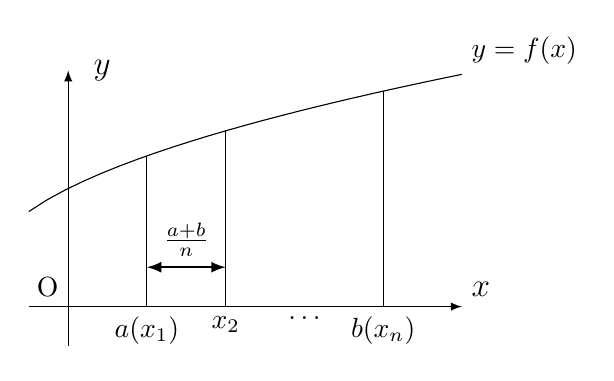
\begin{tikzpicture}
      \path[draw,->,>=latex] (-0.5, 0) -- (5,0) node[above right] {\large $x$};
      \path[draw,->,>=latex] (0, -0.5) -- (0,3) node[right=2mm] {\large $y$} ;
      \path (0,0) node[above left] {$\mathrm{O}$};
      \path[draw,domain=-0.5:5] plot (\x, {sqrt(\x+1)+0.5}) node[above right] {$y=f(x)$};
      \draw [draw] (1,{sqrt(1+1)+0.5}) -- (1,0)node [below] {$a(x_1)$};
      \draw [draw] (2,{sqrt(2+1)+0.5}) -- (2,0)node [below] {$x_2$};
      \draw [draw] (3,0) -- (3,0)node [below] {$\dots$};
      \draw [draw] (4,{sqrt(4+1)+0.5}) -- (4,0)node [below] {$b(x_n)$};
      \draw [thick,latex-latex] (1,0.5) -- (2,0.5) node [above, midway] {$\frac{a+b}{n}$};
\end{tikzpicture}
\caption{合成台形公式のイメージ} 
\label{gtrap}
\end{figure}

表\ref{TrapezoidalRuletable}にTrapezoidalRule関数の機能,引数,返り値の3つを示す.TrapezoidalRule関数は
2点$a$,$b$を$n$分割したときの台形公式による数値積分を求める関数であるから,2点$a$,$b$および分割数$n$を引数,
数値積分の結果を返り値とする設計になっている.

\begin{table}[H]
  \caption{TrapezoidalRule関数の機能,引数,返り値}
  \label{TrapezoidalRuletable}
  \begin{center}
      \begin{tabular}{c|l}\hline
    機能 & 2点$a$,$b$を$n$分割したときの台形公式による数値積分を返す.\\
    引数 & double a,double b,int n\\
    返り値 & double型 \\ \hline
      \end{tabular}
  \end{center}
  \end{table}

  リスト\ref{TrapezoidalRule}にTrapezoidalRule関数のソースコードを示す.リスト\ref{TrapezoidalRule}の2~5行目では分割数$n$が
  不正な値(0や負)である場合にエラーを表示してプログラムを終了する処理を行ってる.ただし,exit関数を用いるためにはstdlib.hをincludeする必要が
  ある.そして,リスト\ref{TrapezoidalRule}の7~11行目では区間[$a$,$b$]を$n$分割して,各区間にTrapezoidal関数を実行する処理を行っている.
  結果はdouble型の引数sumに格納され,returnされる.
      \begin{lstlisting}[basicstyle=\ttfamily\footnotesize, frame=single,label=TrapezoidalRule,caption=TrapezoidalRule関数]
double TrapezoidalRule(double a,double b,int n){
    if(n<=0){
        printf("Incorrect value of n");
        exit(0);
    }

    double sum=0;
    for(double i=0;i<n;i++){
        sum+=Trapezoidal(a+i*(b/n),a+(i+1)*(b/n));
    }
    return sum;
}
            \end{lstlisting}

    \subsubsection{main関数}
    TrapezoidalRule関数を実行し,結果を表示する関数としてmain関数を作成する.リスト\ref{main1}にmain関数のソースコードを示す.
    リスト\ref{main1}の2行目では分割数を1,2,4,$\dots$と細かくするときの上限を定義している.リスト\ref{main1}では
    分割数の上限を256にしている.そして,リスト\ref{main1}の3行目では解析解を定義している.\\
     リスト\ref{main1}の5~11行目では分割数1,2,4,$\dots$,n\_maxについてTrapezoidalRule関数を用いて数学関数$f(x)$の数値積分を
    行い,結果および解析解との誤差の絶対値を表示している.またコメントアウトしている10行目はCSV形式で計算結果を出力するための
    フォーマットである.
      \begin{lstlisting}[basicstyle=\ttfamily\footnotesize, frame=single,label=main1,caption=main1関数]
int main(int argc,char *argv[]){
    int n_max = 256;
    double ans = logf(3)/2;

    double result;
    for(int i=1;i<=n_max;i*=2){
        result = TrapezoidalRule(0,M_PI/6,i);
        printf("n =  %4d  result = %lf  error = %lf\n",i,result,fabs(result-ans));
        // output format for csv
        //printf("%d,%lf,%0.15lf\n",i,result,fabs(result-ans));
    }
    return 0;
}
            \end{lstlisting}

    \subsection{実行結果}
    図\ref{result1}に課題1のプログラムの実行結果を示す.図\ref{result1}において,分割数が1から256についてTrapezoidalRule関数
    を実行できていることがわかる.TrapezoidalRule関数による数値積分の結果についても,解析解$\frac{1}{2} \log_{e} 3 = 0.5493061$
    に十分近い値であることがわかる.解析解に収束する様子や誤差の考察については次節で行う.

    \begin{figure}[H]
      \centering
      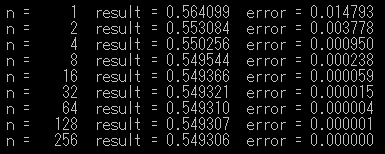
\includegraphics[scale=0.9]{kadai1.png}
      \caption{課題1の実行結果}
       \label{result1}
      \end{figure}

    \subsection{考察}
    !
    
    \section{課題2}
    本章では課題2における課題内容,プログラムの説明,実験結果,考察の4つについて述べる.
    \subsection{課題内容}
    課題2の課題内容はシンプソンの公式を用いて式(\ref{kadai2siki})の数値積分を行うものである.
    解析解は$1$である.
    \begin{equation}
      \int_0^\frac{\pi}{2} \sin x dx
          \label{kadai2siki}
        \end{equation}
    数値積分は次の2点についてプログラムの作成および実行を行い結果を考察する.
    \begin{enumerate}
      \item float型とdouble型のそれぞれで数値積分を行い丸め誤差が現れる刻み幅$h$.
      \item 刻み幅を$\frac{1}{2}$倍ずつ変化させたときの誤差の減少.
      \end{enumerate}

    \subsection{プログラムの説明}
    本節では課題2で作成したプログラムにおいて,次に示す4つの関するの役割
    および機能について説明する.なお,課題2ではdouble型およびfloat型のそれぞれで
    数値積分を行う関数を作成したが,ここではdouble型のプログラムのみ説明する.float
    型のプログラムについては,doubleの部分をfloatに変更すれば問題なく実行できる.
    \begin{enumerate}
      \item func関数
      \item Simpson関数
      \item SimpsonRule関数
      \item main関数
      \end{enumerate}
    
    \subsubsection{func関数}
    func関数は課題1と同様に数値計算を行う数学関数を定義する関数である.
    したがって関数の機能,引数,返り値は表\ref{func1table}と同じである.\\
      リスト\ref{func2}にfunc関数のソースコードを示す.func関数は引数xについて積分を行う数学関数$f(x)=\sin x$
      の値を返す.
      \begin{lstlisting}[basicstyle=\ttfamily\footnotesize, frame=single,label=func2,caption=func関数]
double func(double x){
    return sin(x);
} 
            \end{lstlisting}

    \subsubsection{Simpson関数}
    Simpson関数は数学関数$f(x)$において与えられた2点$a$,$b$におけるシンプソン法による数値積分を行う関数である.
    $a$から$b$までの$f(x)$の積分はシンプソン法により式(\ref{simpleSimpson})のように近似できる.ただし,$h$は積分を行う
    区間の幅である.すなわち$h=\frac{b-a}{2}$である.
    \begin{equation}
      \int_a^b f(x) dx \simeq \frac{h}{3} \left[ f(a)+4f \left( \frac{a+b}{2} \right) +f(b) \right] 
          \label{simpleSimpson}
        \end{equation}
     式(\ref{simpleSimpson})の意味について説明する.台形公式では2点$a$,$b$のおける$f(a)$,$f(b)$の値のみを用いて数値積分
    を行っていた(式(\ref{simpleTrapezaidal}))がさらに精度を高めたい.そこで$a$,$b$の中点$\frac{a+b}{2}$の値を用いて2
    次の近似を行う.3点における$f(x)$の値をそれぞれ$y_0,y_1,y_2$とする.このとき,$\frac{h}{2}$を基準とすると,3点は$(-h,y_0),(0,y_1),(h,y_2)$
    と表せる.$f(x)$を近似する2次多項式$y=a+bx+cx^2$とおくと式(\ref{startr})~式(\ref{endr})の連立方程式が得られる.
    \begin{numcases}
      {}
      \label{startr}
      a-bh+ch^2= y_0 & \\
      a = y_0 & \\
      \label{betweenr}
      a+bh+ch^2=y_2
      \label{endr} 
    \end{numcases}
      式(\ref{startr})$+$式(\ref{betweenr})$\times 4$+式(\ref{endr})を計算すると式(\ref{forsimp})が得られる.これを
      面積$S$の計算に用いることでシンプソン法の式(\ref{simpleSimpson})が得られる.
    \begin{eqnarray}
      (a-bh+ch^2)+4a+(a+bh+ch^2) &=& y_0 +4y_1+y_2 \\
      6a+2ch^2 &=& y_0 +4y_1+y_2 
      \label{forsimp}
    \end{eqnarray}
     求めたい面積$S$を2次多項式の近似で計算すると式(\ref{forsimp2})のようにシンプソン法の式(\ref{simpleSimpson})
    が得られる.式(\ref{forsimp2})の計算において,式(\ref{tmp1})から式(\ref{forsimp2})の計算には式(\ref{forsimp})
    を用いている.

    \begin{eqnarray}
      S &=& \int_{-h}^{h} (a+bx+cx^2) dx \\
      &=& 2 \int_{0}^{h} (a+cx^2) dx \\
      &=& 2 \left[ ax+\frac{cx^3}{3} \right]_0^h \\
      &=& \frac{h}{3}(6a+2ch^2) \label{tmp1}\\
      &=& \frac{h}{3} \left[ f(a)+4f \left( \frac{a+b}{2} \right) +f(b) \right] 
      \label{forsimp2}
    \end{eqnarray}
    
    表\ref{Simpsontable}にSimpson関数の機能,引数,返り値の3つを示す.Simpson関数は2点$a$,$b$における
    シンプソン法による数値積分を行う関数であるから,2点$a$,$b$を引数,数値積分の結果を返り値とする設計になっている.
    \begin{table}[H]
      \caption{Simpson関数の機能,引数,返り値}
      \label{SimpsonTtable}
      \begin{center}
          \begin{tabular}{c|l}\hline
        機能 & 2点$a$,$b$におけるシンプソン法による数値積分を返す.\\
        引数 & double a,double b\\
        返り値 & double型 \\ \hline
          \end{tabular}
      \end{center}
      \end{table}

      リスト\ref{Simpson}にSimpson関数のソースコードを示す.Simpson関数は引数$a$,$b$について式(\ref{simpleSimpson})
      の計算結果を返す.
      \begin{lstlisting}[basicstyle=\ttfamily\footnotesize, frame=single,label=Simpson,caption=Simpson関数]
double Simpson(double a,double b){
    double h = (b-a)/2;
    double c = (a+b)/2;
    return h*(func(a)+4*func(c)+func(b))/3;
}
      \end{lstlisting}

    \subsubsection{SimpsonRule関数}
    SimpsonRule関数は区間[$a$,$b$]を$n$個に分割して,分割した区間のそれぞれにシンプソン法による数値積分を適用する関数である.
    区間を分割して積分を行うイメージとしてはTrapezoidalRule関数と同様である.\\
     表\ref{SimpsonRuletable}にSimpsonRule関数の機能,引数,返り値の3つを示す.SimpsonRule関数は
    2点$a$,$b$を$n$分割したときのシンプソン法による数値積分を求める関数であるから,2点$a$,$b$および分割数$n$を引数,
    数値積分の結果を返り値とする設計になっている.

    \begin{table}[H]
      \caption{SimpsonRule関数の機能,引数,返り値}
      \label{SimpsonRuleTtable}
      \begin{center}
          \begin{tabular}{c|l}\hline
        機能 & 2点$a$,$b$を$n$分割したときのシンプソン法による数値積分を返す.\\
        引数 & double a,double b,int n\\
        返り値 & double型 \\ \hline
          \end{tabular}
      \end{center}
      \end{table}

      リスト\ref{SimpsonRule}にSimpsonRule関数のソースコードを示す.
      リスト\ref{SimpsonRule}の2~5行目では分割数$n$が不正な値(0や負)である場合にエラーを表示してプログラムを終了する処理を行ってる.
      そして,リスト\ref{SimpsonRule}の6~11行目では区間[$a$,$b$]を$n$分割して,各区間にSimpson関数を実行する処理を行っている.結果はdouble型の引数sumに格納され,returnされる.
      \begin{lstlisting}[basicstyle=\ttfamily\footnotesize, frame=single,label=SimpsonRule,caption=SimpsonRule関数]
double SimpsonRule(double a,double b,int n){
    if(n<=0){
        printf("Incorrect value of n");
        exit(0);
    }
    double sum=0;
    for(double i=0;i<n;i++){
        sum+=Simpson(a+i*(b/n),a+(i+1)*(b/n));
    }
    return sum;
}
            \end{lstlisting}

    \subsubsection{main関数}
    SimpsonRule関数を実行し,結果を表示する関数としてmain関数を作成する.リスト\ref{main2}にmain関数のソースコードを示す.
    リスト\ref{main2}の2行目では分割数を1,2,4,$\dots$と細かくするときの上限を定義している.リスト\ref{main2}では
    分割数の上限を256にしている.
     リスト\ref{main2}の3~7行目では分割数1,2,4,$\dots$,n\_maxについてSimpsonlRule関数を用いて数学関数$f(x)$の数値積分を
    行い,結果(少数以下16桁)および解析解との誤差の絶対値を表示している.ただし解析解3.141592はオブジェクト形式マクロで定義している.
      \begin{lstlisting}[basicstyle=\ttfamily\footnotesize, frame=single,label=main2,caption=main2関数]
int main(int argc,char *argv[]){
    int n_max = 256;
    for(int i=1; i<=n_max; i*=2){
        double result = SimpsonRule(0,M_PI/2,i);
        printf("split = %4d   result = %1.16lf   error = %1.16lf\n",
        i,result,fabs((double)1-result));
    }
    return 0;
}
    \end{lstlisting}

    \subsection{実行結果}
    図\ref{kadai2d}に課題2のプログラムのdouble型における実行結果,図\ref{kadai2f}にfloat型における実行結果を示す.
    図\ref{kadai2d}および図\ref{kadai2f}において分割数1から256についてSimpsonRule関数を実行できていることがわかる.
    どちらの実行結果においても数値積分の結果が1に収束していることが読み取れる.解析解に収束する様子や誤差の考察は次節で行う.
    \begin{figure}[H]
      \centering
      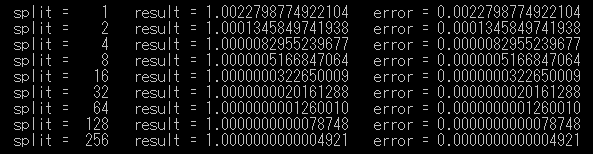
\includegraphics[scale=0.9]{kadai2double.png}
      \caption{課題2の実行結果(double型)}
       \label{result2d}
      \end{figure}

      \begin{figure}[H]
        \centering
        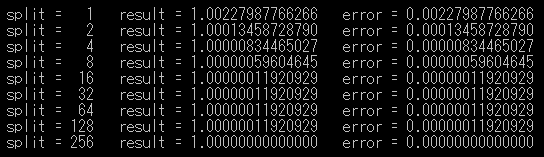
\includegraphics[scale=0.9]{kadai2float.png}
        \caption{課題2の実行結果(float型)}
         \label{result2f}
        \end{figure}

    \subsection{考察}

    \section{課題3}
    本章では課題3における課題内容,プログラムの説明,実験結果,考察の4つについて述べる.
    \subsection{課題内容}
    \subsection{プログラムの説明}
    \subsection{実行結果}
    \subsection{考察}

    \section{課題4}
    本章では課題4における課題内容,プログラムの説明,実験結果,考察の4つについて述べる.
    \subsection{課題内容}
    \subsection{プログラムの説明}
    \subsection{実行結果}
    \subsection{考察}

    \section{課題5}
    本章では課題5における課題内容,プログラムの説明,実験結果,考察の4つについて述べる.
    \subsection{課題内容}
    \subsection{プログラムの説明}
    \subsection{実行結果}
    \subsection{考察}

        \begin{thebibliography}{9}
          \bibitem{NNCT}  国立高専機構長野高専,閲覧日2020年8月7日
          \end{thebibliography}

\end{document}

